\documentclass[11pt,a4paper]{article}

\usepackage[utf8]{inputenc}
\usepackage[T1]{fontenc}
\usepackage[spanish,es-tabla]{babel}
\usepackage{lmodern}
\usepackage[margin=2.5cm]{geometry}
\usepackage{amsmath,amssymb}
\usepackage{graphicx}
\usepackage{booktabs}
\usepackage{array}
\usepackage{multirow}
\usepackage{caption}
\usepackage{float}
\usepackage{microtype}
\usepackage{xcolor}
\usepackage[colorlinks=true,linkcolor=blue!50!black,citecolor=blue!50!black,urlcolor=blue!50!black]{hyperref}

\captionsetup{font=small,labelfont=bf}
\setlength{\parskip}{0.4em}

\title{\textbf{Predicción de demanda de pasajeros en transporte urbano a 30, 60 y 120 minutos con datos de sensores y gradient boosting}\\[0.4em]
\large Caso de tres rutas de SOBUSA (2023--2025)}

\author{Daza Roger: \texttt{polora@uninorte.edu.co}\\
Del Sole Matteo: \texttt{msole@uninorte.edu.co}\\
Romero Rafael: \texttt{arafaelr@uninorte.edu.co}\\[0.3em]
\small Universidad del Norte, Barranquilla}

\date{\today}

\begin{document}
\maketitle

\begin{abstract}
Anticipar cuántos pasajeros subirán a un bus en las próximas horas permite ajustar la oferta de viajes antes de que se produzca el desajuste. En este trabajo se construye un sistema de predicción de las subidas de pasajeros por ruta en franjas de 15 minutos, con horizontes de 30, 60 y 120 minutos, para tres rutas del operador SOBUSA. Se usan 176 millones de lecturas de sensores de conteo (2023--2025), a las que se aplican reglas de calidad derivadas de un análisis exploratorio: días sin lecturas, saltos del contador y un sensor de bajadas poco fiable. Se entrena un modelo LightGBM con objetivo de Poisson por horizonte, elegido frente a otras cinco variantes de gradient boosting y ajustado con búsqueda bayesiana y validación temporal, con 22 variables que usan únicamente información disponible en el instante de predecir, lo cual se verifica con una prueba de alteración del futuro. En un periodo de prueba posterior al de entrenamiento (mayo a noviembre de 2025), el modelo reduce el WAPE de 14,9\,\% (promedio de las cuatro semanas previas) a 10,1\,\%, 10,5\,\% y 10,8\,\% para los horizontes de 30, 60 y 120 minutos. Un intervalo del 80\,\% obtenido con regresión por cuantiles y calibración conforme cubre entre 81,6\,\% y 82,5\,\% de las observaciones. La mejora proviene sobre todo del uso de tres años de datos limpios de sensores; la elección entre familias de gradient boosting cambia el error en décimas de punto. En días especiales el error sube a 14--16\,\%, frente a 99\,\% de la línea base. El sistema se despliega como un servicio con actualización incremental diaria, recomendación de frecuencia, alertas y reentrenamiento controlado frente al modelo activo.
\end{abstract}

\noindent\textbf{Palabras clave:} predicción de demanda, transporte público, series de tiempo, LightGBM, predicción conforme, conteo de pasajeros.

%-----------------------------------------------------------------------
\section{Introducción}
%-----------------------------------------------------------------------

La demanda de pasajeros en el transporte público urbano sigue patrones regulares (picos de la mañana y de la tarde, diferencias entre días hábiles y fines de semana), pero también sufre alteraciones que el calendario no siempre anuncia: festivos, Carnaval, partidos de la selección nacional, lluvias o paros. Un operador que conoce con antelación la demanda esperada puede reforzar o reducir viajes, y evaluar si la programación del día se ajusta a lo que ocurre en la calle.

Este trabajo aborda el problema de predecir, para cada ruta, el número de pasajeros que suben en una franja de 15 minutos con una antelación de 30, 60 y 120 minutos. Los datos provienen del reto de datos de SOBUSA e incluyen las lecturas de los sensores de pasajeros de los buses entre enero de 2023 y diciembre de 2025.

Las contribuciones son las siguientes:
\begin{enumerate}
  \item Un diagnóstico de calidad de los datos de sensores que identifica tres problemas concretos (días sin lecturas, saltos del contador y bajadas inconsistentes) y las reglas para tratarlos.
  \item Un conjunto de 22 variables sin fuga de información, con una prueba directa que comprueba que ninguna usa datos posteriores a la referencia de predicción.
  \item Un modelo por horizonte que mejora entre 27\,\% y 32\,\% el error de la mejor línea base, con una comparación de seis variantes de gradient boosting y una ablación que cuantifica el aporte de cada grupo de variables.
  \item Un intervalo de confianza del 80\,\% calibrado con predicción conforme, que alcanza la cobertura nominal en las tres rutas.
  \item Un servicio que sirve los modelos con el mismo código de variables del entrenamiento, se actualiza a diario y solo reemplaza al modelo activo cuando un candidato lo supera en días que ninguno de los dos vio.
\end{enumerate}

%-----------------------------------------------------------------------
\section{Datos}
%-----------------------------------------------------------------------

\subsection{Fuentes}

Se revisaron las 30 tablas de la base de datos del operador. La fuente principal es la tabla \texttt{conteo\_pasajeros\_destino}, que guarda la lectura del sensor de pasajeros de cada bus aproximadamente cada minuto (176 millones de filas entre enero de 2023 y diciembre de 2025). Las lecturas se agregan por ruta y por franja de 15 minutos según la hora real de cada subida, no según la hora de salida del bus. Esto es importante porque un viaje dura en promedio unas tres horas (mediana de 198 minutos), de modo que asignar sus pasajeros a la hora de salida desplazaría la demanda.

Como fuentes complementarias se usan la programación de viajes (\texttt{progvehiculos}, 565 mil viajes) y las tablas de calendario con festivos, temporadas (Precarnaval, Carnaval, Semana Santa) y eventos con su porcentaje de impacto declarado. Tras la agregación quedan 243\,508 franjas de 15 minutos con servicio y 43,8 millones de subidas para tres rutas: la Ruta 2 (Silencio), la Ruta 16 (Carrera 54) y la Ruta 21 (Calle 72).

La tabla \texttt{timbradas\_segmentos}, que daba subidas por segmento de 500 m, se descartó como fuente del modelo por dos razones (su lógica de asignación a segmentos sí se reutiliza para medir la carga por tramo, Sección~\ref{sec:segmentos}). Solo cubre ocho semanas (1 de enero a 27 de febrero de 2023) y sus horas están desplazadas respecto de los sensores y los despachos: la correlación franja a franja entre ambas fuentes sube de 0,47 a 0,71 al correr los sensores dos horas. En una comparación de totales diarios, las dos fuentes difieren en menos de 1\,\% para la Ruta 16, y la suma de lecturas del sensor por viaje tiene correlación de 0,9999 con el número de pasajeros registrado en la programación, lo que respalda la fiabilidad de los sensores como fuente.

\subsection{Calidad de los datos}

El análisis exploratorio encontró tres problemas que se tratan antes de modelar.

\paragraph{Días sin lecturas.} El último día de cada mes la tabla de sensores está casi vacía (mediana de 15 lecturas frente a unas 180\,000 en un día normal), aunque los viajes sí se realizaron. Se trata de un hueco de la extracción y no de ausencia de demanda. Un día con menos del 5\,\% de las lecturas habituales de su ruta se marca como \emph{faltante} y no como cero; de lo contrario el modelo aprendería que la demanda desaparece a fin de mes. Afecta a 107 días-ruta.

\paragraph{Lecturas imposibles.} Una lectura de cerca de un minuto registra casi siempre entre 1 y 4 subidas, pero hay 38 franjas (0,016\,\%) con lecturas de miles de subidas, producidas por saltos del contador acumulado (el máximo observado supera las 97\,000 subidas en una lectura). Se descarta toda franja en la que alguna lectura supera 90 subidas, que es más de lo que cabe en un bus.

\paragraph{Bajadas no fiables.} En un recorrido completo bajan tantas personas como suben. Sin embargo, la Ruta 21 registra 2,3 veces más bajadas que subidas en 2023 y 1,8 veces en 2024, y la Ruta 16 un 16\,\% más en 2025. Por ello las bajadas no se usan ni como objetivo ni como variable.

Entre 7\,\% y 9\,\% de los viajes programados se cancelan cada año, pero esto no afecta al objetivo, pues los sensores solo registran viajes realizados.

\subsection{Patrones de la demanda}

\paragraph{Tendencia.} La demanda cae entre 3\,\% y 9\,\% por año en las tres rutas (Figura~\ref{fig:tendencia}); a la vez disminuyen los viajes por día y los pasajeros por viaje. Un modelo basado en árboles no extrapola tendencias, por lo que necesita una variable de nivel reciente para no quedar anclado al nivel de 2023.

\begin{figure}[H]
  \centering
  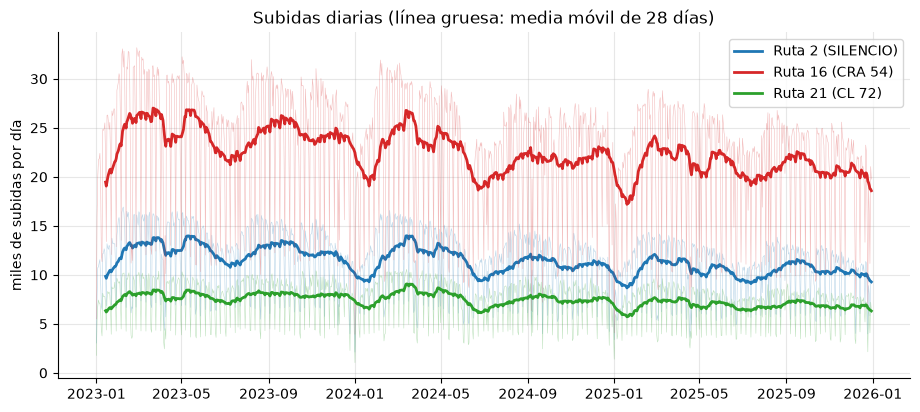
\includegraphics[width=0.85\textwidth]{fig/tendencia.png}
  \caption{Subidas diarias por ruta, 2023--2025. La línea gruesa es la media móvil de 28 días.}
  \label{fig:tendencia}
\end{figure}

\paragraph{Estacionalidad anual.} Una vez quitada la tendencia, enero, junio--julio y diciembre quedan por debajo del promedio (vacaciones escolares y universitarias), y febrero--mayo y agosto--septiembre por encima. La forma se repite los tres años, lo que justifica incluir el día del año y la demanda de la misma franja 52 semanas antes.

\paragraph{Patrón semanal y calendario.} El sábado equivale a 81\,\% de un día hábil, el domingo a 46\,\% y un festivo a 41\,\%. Los días centrales de Carnaval (lunes y martes) dejan la demanda en 35--42\,\% de lo normal y se comportan como festivo; la Semana Santa la deja en 51--60\,\%. El Precarnaval, en cambio, la \emph{aumenta} entre 5\,\% y 24\,\%. Las fiestas patronales no mueven la demanda de estas rutas. En su ventana horaria, los partidos de la selección reducen la demanda entre 17\,\% y 37\,\%, y la Guacherna entre 6\,\% y 19\,\%.

\paragraph{Perfil dentro del día.} Los días hábiles tienen dos picos (6--7 h y 17 h); el fin de semana el pico de la mañana se aplana y se desplaza (Figura~\ref{fig:perfil}). La forma cambia con la ruta y el tipo de día.

\begin{figure}[H]
  \centering
  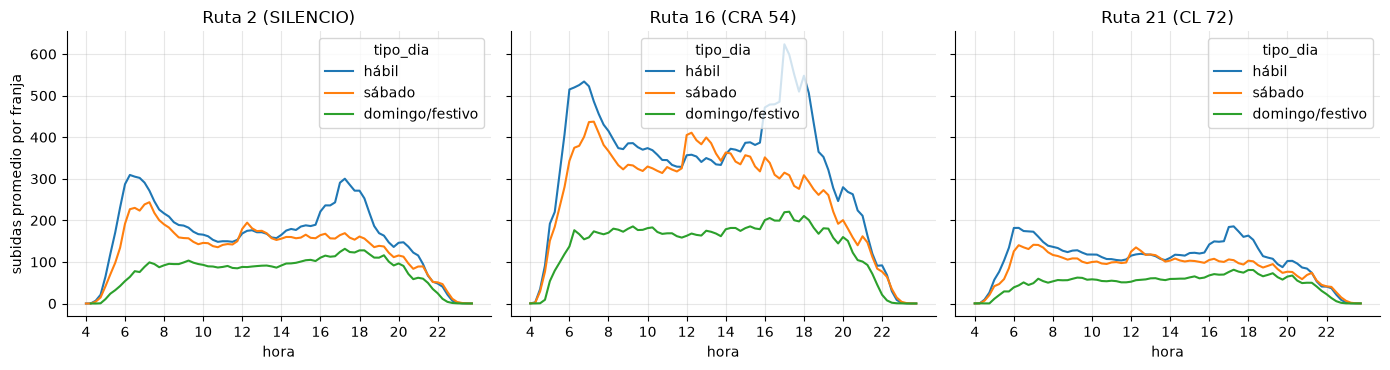
\includegraphics[width=\textwidth]{fig/perfil.png}
  \caption{Subidas promedio por franja de 15 minutos según la hora y el tipo de día, para cada ruta.}
  \label{fig:perfil}
\end{figure}

\paragraph{Qué información predice mejor.} La Tabla~\ref{tab:corr} muestra la correlación de las subidas de una franja con el dato de distintos rezagos. A 30 minutos el dato más reciente (0,82--0,89) vale tanto como el promedio de cuatro semanas (0,83--0,88); a dos horas el dato reciente casi pierde su valor (0,31--0,43) y domina el patrón habitual. El dato de un año antes (0,77--0,85) es tan informativo como el de una semana antes, lo que confirma que la estacionalidad anual es real.

\begin{table}[H]
  \centering
  \caption{Correlación entre las subidas de una franja y el dato con distinto rezago, por ruta.}
  \label{tab:corr}
  \small
  \begin{tabular}{lrrrrrrrr}
    \toprule
    Ruta & 15 min & 30 min & 1 h & 2 h & 1 día & 7 días & 364 días & Prom. 4 sem. \\
    \midrule
    2  & 0,932 & 0,867 & 0,671 & 0,311 & 0,720 & 0,833 & 0,841 & 0,880 \\
    16 & 0,947 & 0,893 & 0,749 & 0,432 & 0,691 & 0,836 & 0,846 & 0,882 \\
    21 & 0,881 & 0,815 & 0,651 & 0,369 & 0,632 & 0,760 & 0,767 & 0,832 \\
    \bottomrule
  \end{tabular}
\end{table}

%-----------------------------------------------------------------------
\section{Metodología}
%-----------------------------------------------------------------------

\subsection{Definición del problema}

Sea $y_{r,t}$ el número de subidas en la ruta $r$ durante la franja de 15 minutos que empieza en $t$. Para un horizonte $h \in \{30, 60, 120\}$ minutos, se busca estimar $y_{r,t}$ usando solo información disponible en el instante de referencia $t-h$. Se entrena un modelo independiente por horizonte, $\hat{y}_{r,t} = f_h(\mathbf{x}_{r,t})$, porque la utilidad de cada variable cambia con la antelación.

\subsection{Variables}

Las 22 variables se agrupan en cuatro familias (Tabla~\ref{tab:vars}). Las del calendario pueden mirar la franja $t$ porque se conocen con anticipación. Las que dependen de lo observado usan datos hasta $t-h$ como máximo.

\begin{table}[H]
  \centering
  \caption{Variables del modelo. $h$ es el horizonte expresado en franjas de 15 minutos.}
  \label{tab:vars}
  \small
  \renewcommand{\arraystretch}{1.15}
  \begin{tabular}{p{2.3cm} p{3.6cm} p{8.2cm}}
    \toprule
    Grupo & Variable & Definición \\
    \midrule
    Calendario & \texttt{id\_ruta} & Ruta (2, 16 o 21). \\
     & \texttt{minuto\_dia} & Minuto del día de la franja $t$. \\
     & \texttt{dia\_semana}, \texttt{tipo\_dia} & Día de la semana; hábil, sábado o domingo/festivo (lunes y martes de Carnaval cuentan como festivo). \\
     & \texttt{mes}, \texttt{dia\_del\_anio} & Posición en el año. \\
     & \texttt{es\_festivo}, \texttt{precarnaval}, \texttt{carnaval\_central}, \texttt{semana\_santa} & Indicadores de temporada. \\
     & \texttt{impacto\_evento} & Porcentaje de impacto declarado del evento activo en la franja. \\
    \addlinespace
    Reciente & \texttt{lag\_h}, \texttt{lag\_h\_mas\_1} & Subidas en $t-h$ y $t-h-1$. \\
     & \texttt{media\_1h\_previa} & Media de las cuatro franjas hasta $t-h$. \\
     & \texttt{ratio\_hoy} & Subidas acumuladas del día hasta $t-h$ sobre lo habitual a esa hora (promedio de cuatro semanas). \\
     & \texttt{nivel\_28d} & Subidas medias por franja en los 28 días previos a $t-h$. \\
    \addlinespace
    Estacional & \texttt{lag\_1d}, \texttt{lag\_7d}, \texttt{prom\_4\_semanas} & Misma franja 1 día, 7 días y promedio de 4 semanas antes. \\
     & \texttt{lag\_364d} & Misma franja 52 semanas antes (mismo día de la semana). \\
    \addlinespace
    Oferta & \texttt{viajes\_1h\_previa} & Viajes con lecturas en la última hora hasta $t-h$. \\
     & \texttt{viajes\_habituales} & Viajes en la franja $t$, promedio de cuatro semanas. \\
    \bottomrule
  \end{tabular}
\end{table}

Dos decisiones merecen comentario. Primero, \texttt{nivel\_28d} y \texttt{ratio\_hoy} existen para captar, respectivamente, la caída anual de la demanda y los días atípicos que el calendario no anuncia (lluvia, paros). Segundo, los \emph{viajes programados} de la franja objetivo no se usan: se registran en promedio unos 12 minutos antes de salir (solo 9,3\,\% con 30 minutos o más de anticipación y 0,12\,\% con dos horas o más), así que a 30--120 minutos todavía no existen y usarlos sería fuga de información. En su lugar se emplean los viajes de la última hora conocida y los viajes habituales de esa franja.

Los valores faltantes (por ejemplo, \texttt{lag\_364d} no existe durante el primer año, 37\,\% de las filas) se dejan vacíos y los maneja el modelo de árboles de forma nativa.

\subsection{Verificación de ausencia de fuga temporal}

Además de razonar cada variable, se verifica de forma empírica que ninguna usa el futuro. Se elige un instante de corte $C$, se reemplazan por valores basura todos los datos posteriores a $C$ y se recalculan las variables. Para toda franja objetivo $t$ con referencia $t-h \le C$, ninguna variable debería cambiar. La prueba se repite con cinco cortes aleatorios y los tres horizontes. Como control, se repite con una variable con fuga introducida a propósito (los viajes de la propia franja $t$), que la prueba debe detectar. En todos los casos las 22 variables permanecen idénticas y el control con fuga es detectado.

\subsection{Modelo}

Se usa LightGBM~\cite{ke2017lightgbm} con objetivo de Poisson, apropiado para una variable de conteo no negativa. La elección sale de una comparación previa a 60 minutos, con las mismas variables y la partición de la versión anterior del estudio, entre seis variantes de gradient boosting (Tabla~\ref{tab:familias}). LightGBM con Poisson obtuvo el menor WAPE y la menor desviación de Poisson y entrenó en menos de la mitad del tiempo de XGBoost~\cite{chen2016xgboost}. Las diferencias entre las variantes de árboles con objetivo de conteo son de centésimas de punto; el GradientBoosting clásico de scikit-learn, con pérdida cuadrática, queda claramente detrás. XGBoost se sigue entrenando en cada ejecución como referencia.

\begin{table}[H]
  \centering
  \caption{Comparación de familias de gradient boosting a 60 minutos (WAPE y desviación de Poisson en prueba, partición de la versión anterior).}
  \label{tab:familias}
  \small
  \begin{tabular}{lrrr}
    \toprule
    Modelo & WAPE & Desv. Poisson & Segundos \\
    \midrule
    LightGBM, Poisson (elegido) & 10,69\,\% & 3,954 & 11 \\
    LightGBM, Poisson con variables categóricas & 10,69\,\% & 3,978 & 13 \\
    LightGBM, Tweedie ($p=1{,}3$) & 10,72\,\% & 4,001 & 7 \\
    XGBoost, Poisson & 10,73\,\% & 3,977 & 24 \\
    HistGradientBoosting (scikit-learn), Poisson & 10,81\,\% & 4,013 & 41 \\
    GradientBoosting clásico (scikit-learn) & 11,04\,\% & 4,595 & 222 \\
    \bottomrule
  \end{tabular}
\end{table}

Los hiperparámetros se ajustan por horizonte con Optuna~\cite{akiba2019optuna} (muestreador TPE con semilla fija, 15 ensayos), minimizando la desviación de Poisson media en una validación \emph{walk-forward} de cuatro pliegues construida sobre instantes únicos, de modo que las tres rutas de un mismo instante quedan del mismo lado y la validación es siempre posterior al entrenamiento. El espacio de búsqueda incluye la tasa de aprendizaje, el número de hojas, el mínimo de datos por hoja, el submuestreo de variables y de filas y la regularización L2; el primer ensayo es la configuración base, de modo que el ajuste nunca empeora el resultado. El ajuste usa solo datos anteriores al periodo de prueba y reduce la desviación de validación cruzada en 1,1\,\%, 1,9\,\% y 3,1\,\% para 30, 60 y 120 minutos. El número de árboles (hasta 3000) se fija por parada temprana con 100 rondas de paciencia sobre el conjunto de validación: 2561, 1932 y 1868 para los tres horizontes. La semilla es 42 y el entrenamiento es determinista.

\subsection{Intervalo de confianza}

Además de la predicción puntual se entrenan tres modelos LightGBM con pérdida cuantílica para los cuantiles 0,1, 0,5 y 0,9. Un intervalo entre los cuantiles 0,1 y 0,9 suele cubrir menos del 80\,\% nominal, porque los cuantiles se estiman con error. Por eso se aplica regresión cuantílica conformalizada (CQR)~\cite{romano2019conformalized}: en el periodo de validación se calcula, para cada observación, cuánto se sale del intervalo, y el cuantil $\lceil (n+1)\,0{,}8 \rceil / n$ de esas distancias se suma a ambos lados. Bajo intercambiabilidad esto garantiza la cobertura marginal. Se compara con los cuantiles sin calibrar y con un intervalo de ancho constante (el cuantil 0,8 del error absoluto en validación) mediante la cobertura, el ancho medio y el \emph{interval score}~\cite{gneiting2007strictly}, que penaliza tanto el ancho como las observaciones que quedan fuera. En las franjas sin servicio habitual, donde los modelos cuantílicos extrapolan, el intervalo se reduce a la predicción puntual más o menos el ajuste conforme y se marca como no calibrado.

\subsection{Partición temporal y líneas base}

El entrenamiento usa los datos hasta el 30 de noviembre de 2025; diciembre se reserva para demostrar la actualización incremental (Sección~\ref{sec:despliegue}). La partición es cronológica, calculada sobre el rango que tiene ambas líneas base: 70\,\% para entrenamiento (hasta el 19 de enero de 2025), 10\,\% para validación y 20\,\% para prueba (del 5 de mayo al 29 de noviembre de 2025). La validación se usa para la parada temprana y para calibrar el intervalo, de modo que el periodo de prueba queda intacto. Quedan 165\,694 filas de entrenamiento, 22\,351 de validación y 44\,626 de prueba.

Una vez evaluado, cada modelo se reentrena con todas las franjas válidas hasta el corte (236\,009), con el número de árboles que eligió la parada temprana; lo mismo se hace con los tres modelos cuantílicos. Ese modelo final es el que se despliega. Las métricas que se reportan son las del modelo evaluado, porque el modelo final incluye el periodo de prueba entre sus datos de entrenamiento.

Se comparan cuatro métodos: (i) la \emph{semana pasada}, que repite el valor de la misma franja siete días antes; (ii) el \emph{promedio de cuatro semanas} de la misma franja y día de la semana; (iii) XGBoost con las mismas variables y la misma partición; y (iv) el modelo LightGBM.

\subsection{Métricas}

Se reportan cuatro métricas~\cite{hyndman2006another}:
\begin{align}
\mathrm{MAE} &= \frac{1}{n}\sum_i |y_i-\hat y_i|, &
\mathrm{RMSE} &= \sqrt{\frac{1}{n}\sum_i (y_i-\hat y_i)^2},\\
\mathrm{WAPE} &= \frac{\sum_i |y_i-\hat y_i|}{\sum_i |y_i|}, &
\mathrm{sMAPE} &= \frac{1}{n}\sum_i \frac{2|\hat y_i-y_i|}{|y_i|+|\hat y_i|}.
\end{align}
El WAPE es la métrica principal porque es interpretable (porcentaje del volumen total) y no se dispara en las franjas de poca demanda, como sí lo haría el MAPE. Se reporta además la desviación de Poisson, que es la pérdida que corresponde al objetivo de conteo. Para la importancia de las variables se usan las contribuciones por árbol de LightGBM, que son valores SHAP exactos para modelos de árboles~\cite{lundberg2017unified}; la misma descomposición explica cada predicción individual del servicio. Los residuos se examinan con las pruebas de Ljung-Box~\cite{ljung1978measure} (autocorrelación) y de McLeod-Li~\cite{mcleod1983diagnostic} (varianza cambiante) en rezagos de una hora y de un día.

%-----------------------------------------------------------------------
\section{Resultados}
%-----------------------------------------------------------------------

\subsection{Desempeño en el conjunto de prueba}

La Tabla~\ref{tab:resultados} resume el desempeño. El modelo supera a las dos líneas base en todas las métricas y en los tres horizontes. Respecto del promedio de cuatro semanas, reduce el WAPE 32\,\% a 30 minutos y 27\,\% a 120 minutos. El error crece de forma suave con el horizonte, de 10,1\,\% a 10,8\,\%, lo que indica que la información histórica sostiene la predicción cuando el dato reciente pierde valor. Frente a XGBoost la ventaja es de una décima de punto o menos, en línea con la comparación de familias: con estos datos y variables, la elección del algoritmo de boosting pesa poco.

\begin{table}[H]
  \centering
  \caption{Desempeño en el conjunto de prueba (5 de mayo a 29 de noviembre de 2025). Las líneas base no dependen del horizonte. En negrita, el mejor valor por horizonte.}
  \label{tab:resultados}
  \small
  \begin{tabular}{llrrrrr}
    \toprule
    Horizonte & Método & MAE & RMSE & WAPE & sMAPE & Desv. Poisson \\
    \midrule
    \multirow{2}{*}{---}
      & Semana pasada      & 30,83 & 52,80 & 18,4\,\% & 26,2\,\% & 21,55 \\
      & Promedio 4 semanas & 24,93 & 41,27 & 14,9\,\% & 22,2\,\% & 8,43 \\
    \midrule
    \multirow{2}{*}{30 min}
      & XGBoost  & 17,03 & 26,15 & 10,2\,\% & 19,4\,\% & 3,66 \\
      & LightGBM & \textbf{16,90} & \textbf{25,82} & \textbf{10,1\,\%} & \textbf{19,3\,\%} & \textbf{3,57} \\
    \midrule
    \multirow{2}{*}{60 min}
      & XGBoost  & 17,67 & \textbf{26,67} & 10,5\,\% & 19,7\,\% & \textbf{3,83} \\
      & LightGBM & \textbf{17,63} & 26,73 & \textbf{10,5\,\%} & \textbf{19,6\,\%} & 3,85 \\
    \midrule
    \multirow{2}{*}{120 min}
      & XGBoost  & 18,20 & \textbf{28,21} & 10,9\,\% & 20,0\,\% & \textbf{4,22} \\
      & LightGBM & \textbf{18,19} & 28,29 & \textbf{10,8\,\%} & \textbf{19,9\,\%} & 4,23 \\
    \bottomrule
  \end{tabular}
\end{table}

\subsection{Intervalo de confianza}

La Tabla~\ref{tab:intervalos} compara los tres intervalos. Los cuantiles sin calibrar cubren 77,5--78,2\,\%, por debajo del 80\,\% nominal. La calibración conforme lleva la cobertura a 81,6--82,5\,\% con un ancho apenas mayor y el mismo \emph{interval score}. El intervalo de ancho constante también cubre el 80\,\%, pero su \emph{interval score} es entre 9\,\% y 10\,\% peor, porque usa el mismo ancho a toda hora en lugar de ensancharse cuando la demanda es alta. Por ruta, la cobertura del intervalo calibrado va de 79,5\,\% (Ruta 16) a 84,7\,\% (Ruta 2).

\begin{table}[H]
  \centering
  \caption{Intervalo del 80\,\% en el conjunto de prueba: cobertura, ancho medio (pasajeros por franja) e \emph{interval score} (menor es mejor).}
  \label{tab:intervalos}
  \small
  \begin{tabular}{llrrr}
    \toprule
    Horizonte & Método & Cobertura & Ancho medio & Interval score \\
    \midrule
    \multirow{3}{*}{30 min} & Cuantiles sin calibrar & 77,5\,\% & 52,5 & 77,9 \\
     & Cuantiles + CQR & 81,6\,\% & 55,8 & \textbf{77,8} \\
     & Ancho constante & 81,1\,\% & 53,3 & 84,7 \\
    \midrule
    \multirow{3}{*}{60 min} & Cuantiles sin calibrar & 77,6\,\% & 54,0 & 81,3 \\
     & Cuantiles + CQR & 82,0\,\% & 57,8 & \textbf{81,3} \\
     & Ancho constante & 80,9\,\% & 55,0 & 89,3 \\
    \midrule
    \multirow{3}{*}{120 min} & Cuantiles sin calibrar & 78,2\,\% & 55,9 & \textbf{84,6} \\
     & Cuantiles + CQR & 82,5\,\% & 59,9 & 84,7 \\
     & Ancho constante & 81,0\,\% & 56,3 & 93,2 \\
    \bottomrule
  \end{tabular}
\end{table}

\subsection{Aporte de cada grupo de variables}

La ablación por grupos de variables se hizo con XGBoost en la versión anterior del estudio (partición con prueba del 30 de mayo al 30 de diciembre de 2025), agregando un grupo cada vez con $h=60$ minutos (Tabla~\ref{tab:ablacion} y Figura~\ref{fig:ablacion}). Sus conclusiones no dependen del algoritmo, porque las dos familias difieren en centésimas de punto. El punto de partida (A) es el conjunto de 15 variables de una versión anterior del modelo, que se entrenaba solo con las ocho semanas de \texttt{timbradas\_segmentos} y tenía un WAPE cercano a 40\,\%.

\begin{table}[H]
  \centering
  \caption{Ablación a 60 minutos: WAPE en prueba al agregar grupos de variables. \emph{Especial} agrupa festivos, Carnaval y Semana Santa.}
  \label{tab:ablacion}
  \small
  \begin{tabular}{lrrr}
    \toprule
    Conjunto & WAPE total & WAPE normal & WAPE especial \\
    \midrule
    Línea base: promedio 4 semanas & 15,8\,\% & 13,7\,\% & 113,1\,\% \\
    A. Variables del modelo anterior & 11,1\,\% & 11,0\,\% & 15,6\,\% \\
    B. A + estacionalidad anual & 11,3\,\% & 11,2\,\% & 17,1\,\% \\
    C. B + nivel y marcha del día & 10,9\,\% & 10,8\,\% & 16,8\,\% \\
    D. C + oferta (modelo final) & 10,7\,\% & 10,6\,\% & 16,5\,\% \\
    \bottomrule
  \end{tabular}
\end{table}

\begin{figure}[H]
  \centering
  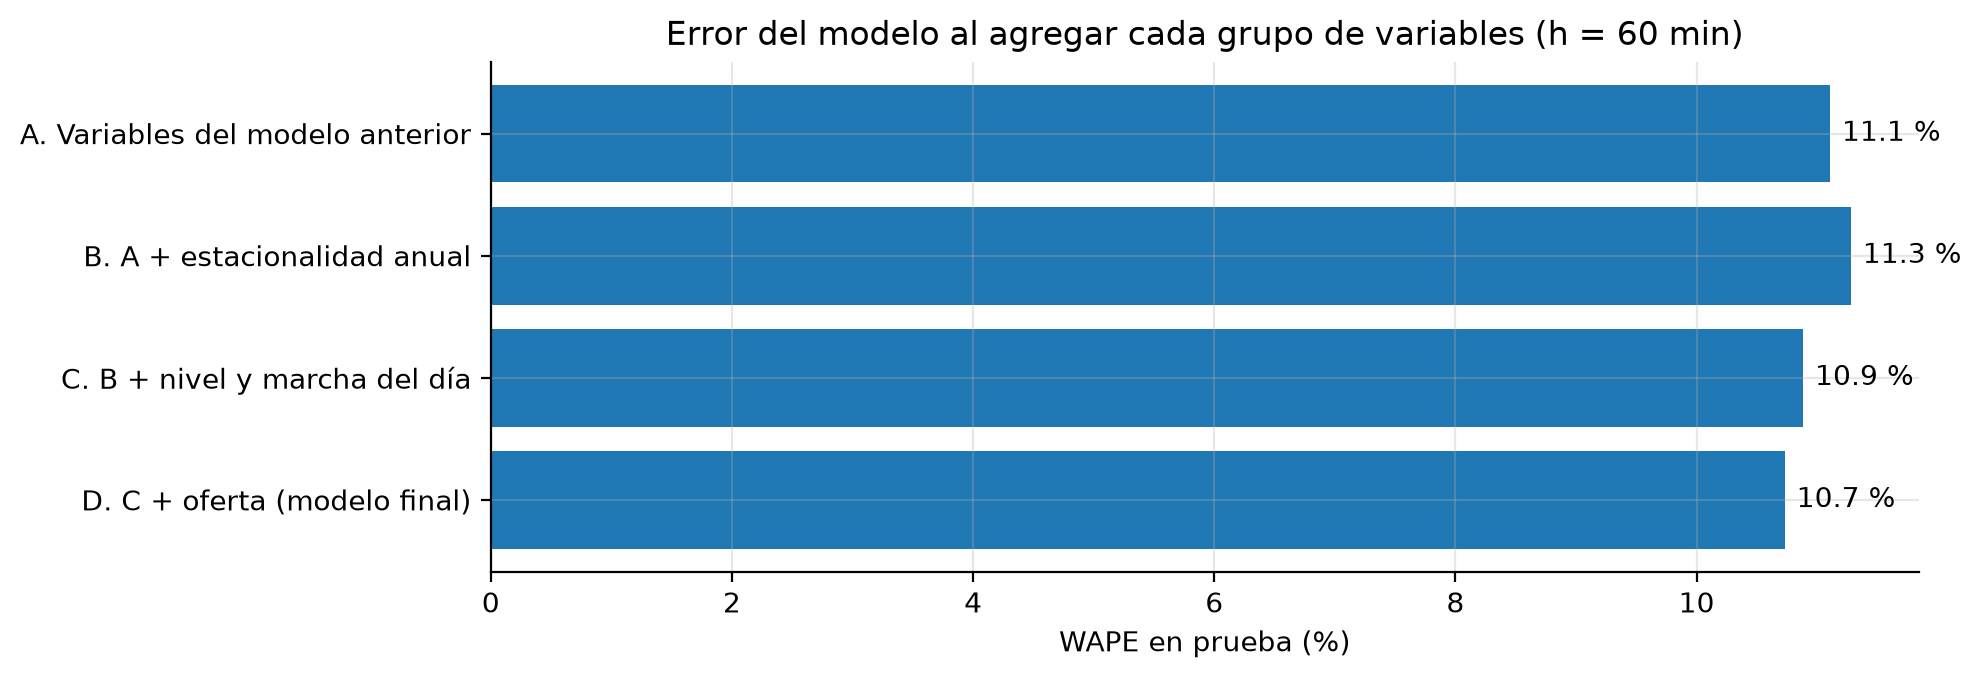
\includegraphics[width=0.85\textwidth]{fig/ablacion.png}
  \caption{Error del modelo (WAPE en prueba, $h=60$ min) al agregar cada grupo de variables.}
  \label{fig:ablacion}
\end{figure}

El resultado principal es que \textbf{la mayor mejora viene de los datos y no de las variables nuevas}: con las mismas 15 variables, pero entrenadas con los tres años de sensores limpios, el WAPE baja de cerca de 40\,\% a 11,1\,\%. Las variables adicionales aportan una mejora pequeña pero consistente, hasta 10,7\,\%. Repetido con tres semillas, el conjunto completo supera al conjunto sin estacionalidad anual en las nueve combinaciones de horizonte y semilla, por 0,06 a 0,10 puntos porcentuales, con una desviación entre semillas de 0,01 a 0,03 puntos. Cabe notar que añadir solo la estacionalidad anual (B) no mejora por sí sola el WAPE total en una sola ejecución; su ventaja aparece en la comparación del conjunto completo repetida con varias semillas. Con LightGBM se probaron además tres grupos candidatos (medias móviles, indicador de hora pico y demanda reciente de las otras rutas): juntos bajan el WAPE de 10,69\,\% a 10,66\,\%, dentro de la variación entre ejecuciones, por lo que no se incorporaron; el último, además, obligaría a predecir las tres rutas a la vez.

\subsection{Importancia de las variables}

La Figura~\ref{fig:shap} muestra la contribución absoluta media de cada variable en el periodo de prueba para los tres horizontes. El promedio de cuatro semanas y la hora del día explican la mayor parte de cada predicción en todos los casos. El último dato conocido (\texttt{lag\_h}) es la segunda variable a 30 minutos, la tercera a 60 y deja de figurar entre las ocho primeras a 120 minutos, donde ganan peso la oferta habitual de viajes y el tipo de día. Esto respalda la decisión de entrenar un modelo por horizonte. Las variables de Carnaval y Precarnaval tienen importancia casi nula únicamente porque el periodo de prueba (mayo a noviembre) no contiene Carnaval. El servicio usa la misma descomposición para explicar cada predicción con sus cinco variables de mayor efecto.

\begin{figure}[H]
  \centering
  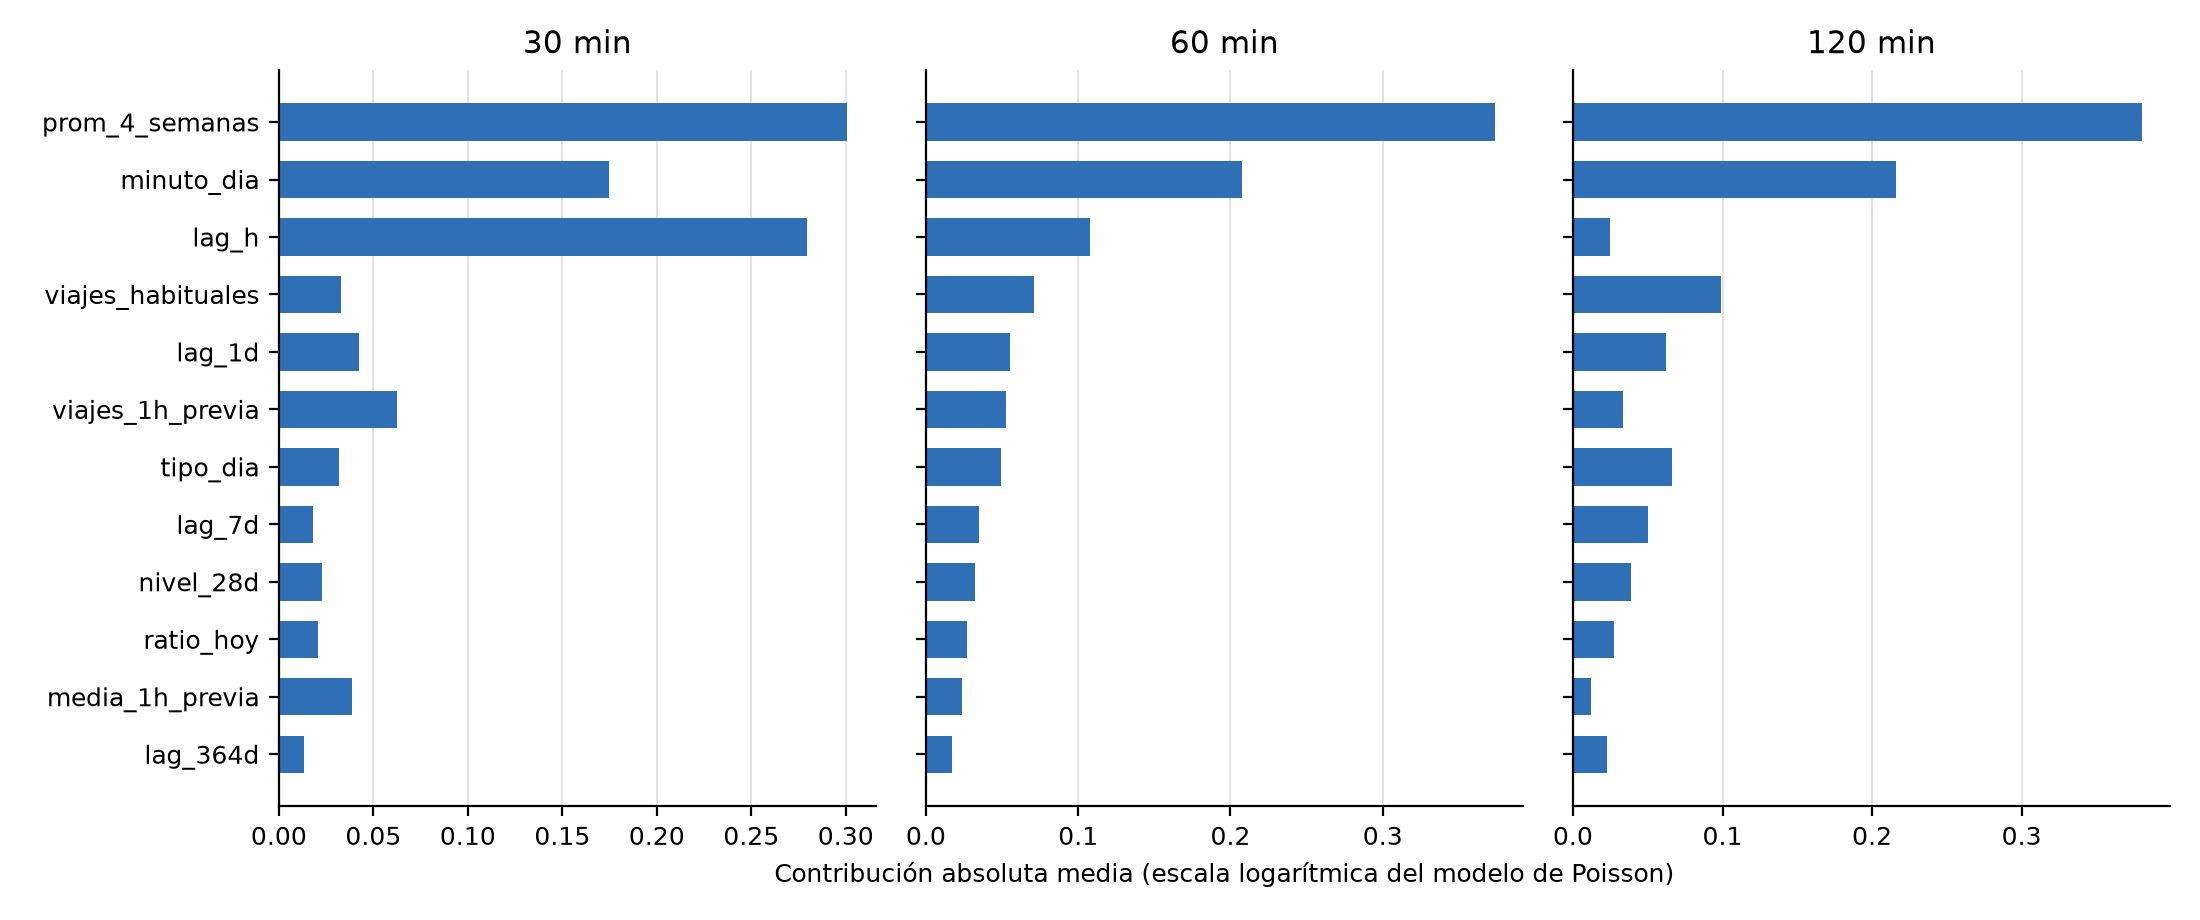
\includegraphics[width=\textwidth]{fig/shap_lgbm.png}
  \caption{Contribución absoluta media de las 12 variables más importantes a 60 minutos (escala logarítmica del modelo de Poisson), para los tres horizontes.}
  \label{fig:shap}
\end{figure}

\paragraph{Residuos y sobreajuste.} Las pruebas de Ljung-Box rechazan la independencia de los residuos en las tres rutas y los tres horizontes, a una hora y a un día; la autocorrelación de primer orden va de 0,17 a 0,38 y crece con el horizonte. McLeod-Li rechaza la varianza constante a una hora en todos los casos. Las predicciones y la cobertura marginal del intervalo siguen siendo válidas, pero los errores de franjas vecinas no son independientes. La brecha entre el error de entrenamiento y el de validación es pequeña (d de Cohen entre 0,12 y 0,16).

\subsection{Resultados por ruta y por tipo de día}

La Tabla~\ref{tab:desglose} desglosa el WAPE de prueba de los mismos modelos de la Tabla~\ref{tab:resultados}.

\begin{table}[H]
  \centering
  \caption{WAPE en prueba por ruta, tipo de día y hora: línea base (promedio de 4 semanas) $\rightarrow$ LightGBM. \emph{Especial} agrupa festivos, Carnaval y Semana Santa (1\,546 franjas); \emph{normal}, 43\,080 franjas. Las horas pico son 6--8 h y 16--18 h.}
  \label{tab:desglose}
  \small
  \begin{tabular}{lccc}
    \toprule
     & 30 min & 60 min & 120 min \\
    \midrule
    Ruta 2 (Silencio)  & 15,4 $\rightarrow$ 10,6\,\% & 15,4 $\rightarrow$ 11,1\,\% & 15,4 $\rightarrow$ 11,4\,\% \\
    Ruta 16 (Cra. 54)  & 13,4 $\rightarrow$ 8,4\,\%  & 13,4 $\rightarrow$ 8,9\,\%  & 13,4 $\rightarrow$ 9,2\,\% \\
    Ruta 21 (Cl. 72)   & 18,6 $\rightarrow$ 14,4\,\% & 18,6 $\rightarrow$ 14,8\,\% & 18,6 $\rightarrow$ 15,2\,\% \\
    \midrule
    Días normales      & 13,3 $\rightarrow$ 10,0\,\% & 13,3 $\rightarrow$ 10,4\,\% & 13,3 $\rightarrow$ 10,8\,\% \\
    Días especiales    & 99,2 $\rightarrow$ 14,3\,\% & 99,2 $\rightarrow$ 15,0\,\% & 99,2 $\rightarrow$ 15,7\,\% \\
    \midrule
    Horas pico         & 14,4 $\rightarrow$ 9,3\,\%  & 14,4 $\rightarrow$ 9,8\,\%  & 14,4 $\rightarrow$ 10,3\,\% \\
    Horas valle        & 15,2 $\rightarrow$ 10,7\,\% & 15,2 $\rightarrow$ 11,1\,\% & 15,2 $\rightarrow$ 11,3\,\% \\
    \bottomrule
  \end{tabular}
\end{table}

\paragraph{Por ruta.} El modelo mejora en las tres rutas y en todos los horizontes. La Ruta 16, la de mayor volumen, es la más predecible (8,4--9,2\,\%); la Ruta 21, la de menor demanda, es la más difícil (14,4--15,2\,\%), probablemente porque con menos pasajeros por franja el ruido relativo es mayor.

\paragraph{Días especiales.} En días normales el error es de 10,0--10,8\,\%. En días especiales sube a 14,3--15,7\,\%, pero la línea base del promedio de cuatro semanas se equivoca en 99,2\,\%: promedia semanas sin festivo y proyecta una demanda de día hábil sobre un día que se comporta como domingo. Esta es la mayor ganancia relativa del modelo y proviene de las variables de calendario y de la marcha del día.

\paragraph{Horas pico.} El error es menor en las horas pico (9,3--10,3\,\%) que en las horas valle (10,7--11,3\,\%), porque en el pico la demanda es más regular y el volumen mayor.

\subsection{Carga por tramo y capacidad}
\label{sec:segmentos}

Para recomendar cuántos buses despachar no basta con las subidas de la hora: importa cuántos pasajeros van a bordo en el tramo más cargado. El operador entregó los scripts que segmentan cada ruta en tramos de 500 m y asignan cada lectura del sensor al segmento más cercano. No pueden ejecutarse sobre la base del reto, que es de solo lectura, y contienen errores que impiden correrlos sin cambios (un punto y coma dentro de un \texttt{CREATE TABLE}, una columna inexistente y un \texttt{ON CONFLICT} que no coincide con la restricción única); además filtran un proceso distinto al de estas rutas, por lo que sus tablas anuales quedaron vacías. Se reprodujo su lógica en la base propia del sistema, con los mismos segmentos (135, 123 y 128 por ruta) y un índice espacial: en dos días de 2023 con datos del operador, las subidas por viaje y segmento coinciden en 99,7\,\% de los 108\,000 pares y los totales son idénticos.

La columna de pasajeros a bordo que calculan los scripts, como diferencia de contadores acumulados, no es utilizable (mediana de 6\,041 ``pasajeros'' por bus), porque los contadores acumulan desde la instalación del equipo. En su lugar se estima la carga balanceando las bajadas de cada viaje para que sumen lo mismo que las subidas. Con las 1,75 millones de lecturas de cuatro semanas de noviembre de 2025 (12\,927 viajes), la mediana del cociente entre la carga máxima y las subidas del viaje es 0,39, 0,43 y 0,37 para las rutas 2, 16 y 21, lo que confirma de forma independiente los factores de carga medidos en el análisis de flota. El tramo más cargado está en la primera mitad del recorrido en la mañana (km 13--20) y en la segunda mitad en la tarde (km 42--46). La carga máxima por viaje tiene un percentil 90 de 49, 56 y 47 pasajeros, y el 9\,\%, 20\,\% y 7\,\% de los viajes supera en algún tramo la capacidad registrada de 50 pasajeros, lo que indica que esa capacidad subestima la carga que los buses realmente llevan.

%-----------------------------------------------------------------------
\section{Despliegue}
\label{sec:despliegue}
%-----------------------------------------------------------------------

Cada modelo se guarda como un paquete (modelo puntual, tres modelos cuantílicos y metadatos: versión de variables, fecha de corte, cortes de validación y prueba, número de árboles, hiperparámetros, semilla y métricas) con la huella SHA-256 de cada archivo, que se verifica al cargarlo, y se registra en una base PostgreSQL propia, separada de la del operador, con un único modelo activo por horizonte. Un servicio FastAPI calcula las variables con la misma función usada para entrenar, de modo que el modelo recibe al predecir exactamente lo que vio al aprender, y rechaza modelos entrenados con otra versión de variables. Para cada consulta entrega la demanda de las ocho franjas siguientes con su intervalo, las cinco variables que más influyeron y una recomendación de buses por hora, intervalo entre despachos y vehículos requeridos, que se dimensiona con el límite superior del intervalo y los parámetros de capacidad, factor de carga, tiempo de ciclo y flota de cada ruta, y que se marca como no viable cuando la flota o el intervalo mínimo no alcanzan. Sobre esa recomendación se evalúan las alertas operativas, con deduplicación e historial.

Un ciclo programado lee de la base del operador, en modo de solo lectura, los datos nuevos desde la última marca de agua, los valida con reglas de calidad, actualiza el histórico, genera predicciones y recomendaciones, vigila el error móvil de siete días del modelo activo y lo reentrena cuando corresponde. El candidato se entrena con los datos nuevos anteriores a una ventana de comparación y compite contra el modelo activo en esa ventana, que ninguno de los dos vio; solo se activa si mejora el WAPE o la desviación de Poisson sin empeorar la otra y supera a la línea base. En la demostración con los primeros días de diciembre de 2025, el error móvil del modelo activo fue de 10,1--11,0\,\%, y un candidato entrenado con cuatro días adicionales lo superó en los tres horizontes (por ejemplo, 10,16\,\% frente a 10,26\,\% a 30 minutos), por lo que fue activado; el modelo anterior queda registrado para poder revertir.

%-----------------------------------------------------------------------
\section{Discusión y limitaciones}
%-----------------------------------------------------------------------

\begin{itemize}
  \item \textbf{Alcance.} El estudio cubre tres rutas; la generalización a otras rutas no está probada.
  \item \textbf{Periodo de prueba sin Carnaval ni Semana Santa.} El desempeño en esas temporadas, las de mayor alteración, no se evaluó fuera de muestra.
  \item \textbf{Errores correlacionados.} El intervalo cubre el 80\,\% de cada franja, pero los errores de franjas vecinas no son independientes, así que la cobertura de una hora completa es menor que la de una franja. Fuera del servicio habitual el intervalo no está calibrado.
  \item \textbf{Capacidad por validar.} La recomendación depende de la capacidad registrada de 50 pasajeros, que la carga medida por tramo supera con frecuencia; el operador debe confirmarla.
\end{itemize}

%-----------------------------------------------------------------------
\section{Conclusiones}
%-----------------------------------------------------------------------

Con tres años de lecturas de sensores correctamente limpiadas y variables sin fuga de información, un LightGBM con objetivo de Poisson predice las subidas de pasajeros por ruta y franja de 15 minutos con un WAPE de 10,1\,\% a 30 minutos, 10,5\,\% a 60 minutos y 10,8\,\% a 120 minutos, entre 27\,\% y 32\,\% mejor que el promedio de las cuatro semanas previas, y con un intervalo del 80\,\% que alcanza su cobertura nominal gracias a la calibración conforme. La conclusión más relevante es práctica: la calidad y la cobertura temporal de los datos pesaron más que la elección del algoritmo o la sofisticación de las variables. El dato reciente es decisivo a 30 minutos, mientras que a 120 minutos domina el patrón habitual, lo que justifica un modelo por horizonte.

%-----------------------------------------------------------------------
\section*{Disponibilidad de datos y código}
%-----------------------------------------------------------------------

El código de extracción, limpieza, entrenamiento, servicio y ciclo incremental, junto con los cuadernos de análisis exploratorio y de ingeniería de variables, está en el repositorio del proyecto \emph{Data Challenge}. Los datos provienen de la base del operador SOBUSA.

\begin{thebibliography}{9}

\bibitem{ke2017lightgbm}
G.~Ke, Q.~Meng, T.~Finley, T.~Wang, W.~Chen, W.~Ma, Q.~Ye y T.-Y.~Liu,
``LightGBM: A highly efficient gradient boosting decision tree'',
en \emph{Advances in Neural Information Processing Systems 30}, 2017.

\bibitem{akiba2019optuna}
T.~Akiba, S.~Sano, T.~Yanase, T.~Ohta y M.~Koyama,
``Optuna: A next-generation hyperparameter optimization framework'',
en \emph{Proc. 25th ACM SIGKDD Int. Conf. on Knowledge Discovery and Data Mining}, 2019, pp.~2623--2631.

\bibitem{romano2019conformalized}
Y.~Romano, E.~Patterson y E.~Candès,
``Conformalized quantile regression'',
en \emph{Advances in Neural Information Processing Systems 32}, 2019.

\bibitem{gneiting2007strictly}
T.~Gneiting y A.~E.~Raftery,
``Strictly proper scoring rules, prediction, and estimation'',
\emph{Journal of the American Statistical Association}, vol.~102, n.º~477, pp.~359--378, 2007.

\bibitem{ljung1978measure}
G.~M.~Ljung y G.~E.~P.~Box,
``On a measure of lack of fit in time series models'',
\emph{Biometrika}, vol.~65, n.º~2, pp.~297--303, 1978.

\bibitem{mcleod1983diagnostic}
A.~I.~McLeod y W.~K.~Li,
``Diagnostic checking ARMA time series models using squared-residual autocorrelations'',
\emph{Journal of Time Series Analysis}, vol.~4, n.º~4, pp.~269--273, 1983.

\bibitem{chen2016xgboost}
T.~Chen y C.~Guestrin,
``XGBoost: A scalable tree boosting system'',
en \emph{Proc. 22nd ACM SIGKDD Int. Conf. on Knowledge Discovery and Data Mining}, 2016, pp.~785--794.

\bibitem{lundberg2017unified}
S.~M.~Lundberg y S.-I.~Lee,
``A unified approach to interpreting model predictions'',
en \emph{Advances in Neural Information Processing Systems 30}, 2017.

\bibitem{hyndman2006another}
R.~J.~Hyndman y A.~B.~Koehler,
``Another look at measures of forecast accuracy'',
\emph{International Journal of Forecasting}, vol.~22, n.º~4, pp.~679--688, 2006.

\end{thebibliography}

\end{document}
